\documentclass{beamer}
\usetheme{metropolis}           % Use metropolis theme
\usepackage[german]{babel}  
\usepackage[utf8]{inputenc}	%dt Sonderzeichen wie ß

\renewcommand*{\figurename}{Abb.}



\title{Varianzanalyse\\\normalsize Cooler Untertitel, den wir uns noch ausdenken}
\date{15. Dezember 2016}
\author{Henri Neumann \& Robert Feldhans}
\institute{Experimentelle Psychologie für Nichtpsychologen}
\begin{document}
	\maketitle
	
	\begin{frame}{Inhalt}
		\setbeamertemplate{section in toc}[sections numbered]
		\tableofcontents[hideallsubsections]
	\end{frame}
	
	\section{Einführung}
	
	%------------
	
	\begin{frame}{Motivation}
		
	\end{frame}
	
	%------------
	
	\begin{frame}{Wiederholung: Was ist Varianz?}
		
	\end{frame}
	
	%------------
	
	\section{Henri}
	
	\section{Robert}
	
	
	%---------------------------------- Ab hier Beispiele für Folien
	
	\section{Historische Einordnung}
	
	\begin{frame}{Beginn des Schlangenöls}
		\begin{columns}[T,onlytextwidth]
			\column{0.7\textwidth}
			\begin{itemize}
				\item aus Mythologie des Wilden Westens
				\item von Wunderheilern eingesetzt
				\item Heilmittel für Gebrechen aller Art
			\end{itemize}
			
			%------------------------ Bilder
			\column{0.3\textwidth}
				
\includegraphics[width=1\textwidth]{Bilder/snakeoil.jpeg}
			%------------------------ Bilder

		\end{columns}
	\end{frame}
	
	\begin{frame}{Schlangenöl allgemein}
		\begin{itemize}
			\item versprochenes Wundermittel
			\item unübersichtliche Bereiche, oft in Technik
			\item \alert{wenig Wirkung}
			\item Heutige Anwendungen oft in Kryptografie und \alert{Antiviren-Software}
		\end{itemize}
	\end{frame}
	
	\section{Malware und ihre Hauptverteilwege}
	
	\begin{frame}{Malware}
		\begin{alertblock}{Malware}
			Software, welche schädliche Funktionen ausführen
		\end{alertblock}
		
		\begin{itemize}
			\item Viren
			\item Würmer
			\item Trojanische Pferde
			\item Ransomware 
			\item ...
			\item \alert{nicht:} fehlerhafte Software
		\end{itemize}
	\end{frame}
	
	\begin{frame}{Verschiedene Malware}
		\begin{alertblock}{Virus}
			Schadprogramm, welches sich verbreitet, in dem es sich in andere Software einschleust. Durch das Kopieren dieser wird der Virus passiv verbreitet (und dabei oft nur lokal)
		\end{alertblock}
		\begin{alertblock}{Wurm}
			Schadprogramm, welches sich aktiv ausbreitet, in dem es Sicherheitsprobleme ausnutzt. Für Nutzer kaum unterschiedlich zu Viren
		\end{alertblock}
		\begin{alertblock}{Trojanisches Pferd}
			Schadprogramm, welches sich als nützliche Anwendung tarnt und ohne Wisse des Anwenders (auch) schädliche Funktionen ausführt
		\end{alertblock}
	\end{frame}
	
	%------------------------ Bilder
	\begin{frame}{Anzahl Malware}
		\begin{figure}
			\centering
			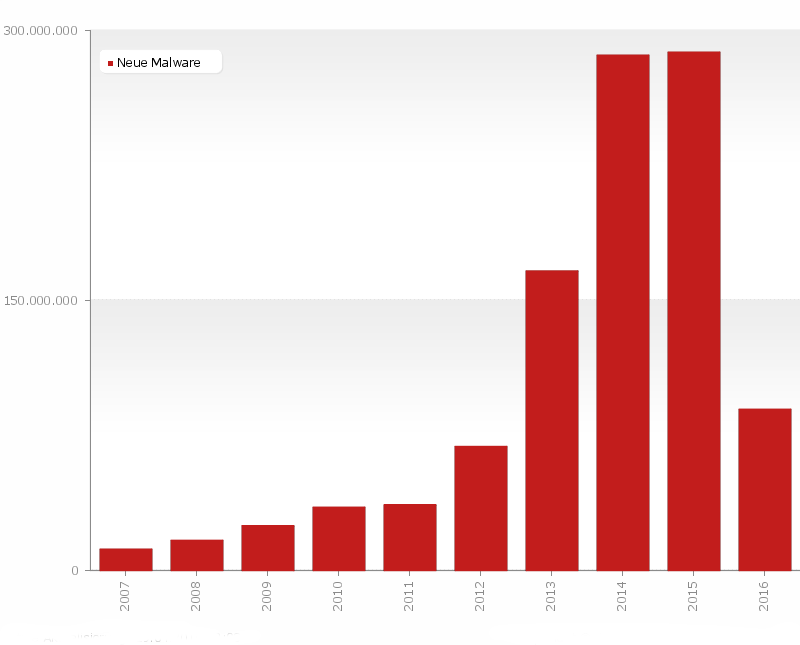
\includegraphics[width=0.7\textwidth]{Bilder/new_malware_transparent.png}
			\caption{Registrierung neuer Schadprogramme in den letzten 10 Jahren. Quelle: avtest}
		\end{figure}		
	\end{frame}
	%------------------------ Bilder
	
	\begin{frame}{Verteilwege von Malware}
		\begin{itemize}
			\item E-Mail-Dateianhänge
			\item Drive-by-Downloads
			\item Datenträger
			\item Netzwerke
		\end{itemize}
	\end{frame}
	
	\begin{frame}{Statistiken}
		\begin{alertblock}{Problem}
			Viele Statistiken zu Malware und ihren Verteilwegen werden von Antiviren-Software-Firmen angeboten
		\end{alertblock}
		\begin{itemize}
			\item wenige \alert{unabhängige} Quellen
			\item Quantität schwer einzuschätzen
			\item nur bekannte Probleme aufgelistet
		\end{itemize}
	\end{frame}
	
	
	\section{Antiviren-Programme}
	
	\begin{frame}{Vermeintliche Lösung}
		\begin{alertblock}{Wie schützen wir uns vor Viren?}
			Wir installieren ein Antiviren-Programm!
		\end{alertblock}
	\end{frame}
	
	\begin{frame}{Verbreitung von AV-Programmen}
		\begin{alertblock}{Zahlen zu AV-Installationen}
			\begin{itemize}
				\item{AVG Antivirus Free (32 \& 64 bit) 22.3M}
				\item{avast Free Antivirus 19.4M}
				\item{Ad-Aware Free Antivirus 9.2M}
			\end{itemize}
			jeweils in Millionen Downloads bei Chip (Windows)
		\end{alertblock}
	\end{frame}

	\subsection{Aufgaben und Vorgehen von AV-Programmen} %----------- Beachte: keine 
	
	\begin{frame}{Virtualisierung I}
		\begin{alertblock}{Virtualisierung}
			Idee: Wir tun nur so, als würden wir verdächtigen Code laufen lassen, überwachen tatsächlich seine Verhaltensweise
		\end{alertblock}
	\end{frame}
	
	
	\begin{frame}{Firewalls I}
		\begin{alertblock}{Firewall}
			Idee: Ein- und ausgehende Kommunikation überwachen, um Kommunikation von Malware zu verhindern/ Malware zu finden\\
		\end{alertblock}
		\begin{alertblock}{Problem}
			Sobald die Kommunikation verschlüsselt abläuft, wird die Überwachung beliebig kompliziert
		\end{alertblock}
	\end{frame}
	
	
	
	\begin{frame}{AV-Browser I}
		\begin{alertblock}{Antiviren-Browser}
			Idee: Wir halten den Nutzer davon ab, schädliche Dateien herunterzuladen, indem wir einen Browser bereitstellen, der gefährliche Websites u.Ä. blockiert
		\end{alertblock}
	\end{frame}
	
	
	\section{Wirksame Maßnahmen gegen Viren}
	
	
	\begin{frame}{Zitat}
		\glqq We cant write secure software. Why are people suprised that we also can not write secure security software?\grqq
	\end{frame}
	
	\begin{frame}[standout]
		Fragen?
	\end{frame}
	
	\appendix
	
	
	\begin{frame}[allowframebreaks]{Quellen}
		\footnotesize
		%\bibliography{demo}
		%\bibliographystyle{abbrv}
		\begin{itemize}
			\item blog.fefe.de
			\item sherpablog.marketingsherpa.com/wp-content/uploads/2016/02/Snake-Oil-Cures-All.jpeg
			\item itwissen.info/definition/lexikon/ (diverse Definitionen)
			\item de.wikipedia.org/wiki/Schadprogramm
			\item av-test.org/de/statistiken/malware/
			\item netmarketshare.com/operating-system-market-share.aspx?qprid=10\&qpcustomd=0
			\item bsi.bund.de/DE/Publikationen/Lageberichte/bsi-lageberichte.html
			%ab hier robads
			\item Chip.de (diverse AV-Downloadseiten)
			\item bugs.chromium.org/p/project-zero/issues/detail?id=769
			\item de.urbandictionary.com/define.php?term=Startkeylogger 
			\item bugs.chromium.org/p/project-zero/issues/detail?id=564\&redir=1
			\item news.softpedia.com/news/avast-safezone-browser-lets-attackers-access-your-filesystem-499990.shtml
			\item imgur.com/Smwnzx3
			\item www.heise.de/security/meldung/Authentifikation-von-McAfees-Enterprise-Security-Manager-loechrig-3036068.html
			\item www.heise.de/security/meldung/Symantec-Endpoint-Protection-Gefaehrlicher-Sicherheitsluecken-Cocktail-2768461.html
			\item thehackernews.com/2015/07/bitdefender-hacked.html?m=1
			\item www.heise.de/mac-and-i/meldung/Apple-Anti-Viren-Apps-fuer-iOS-irrefuehrend-2581916.html
			\item www.heise.de/security/meldung/Antiviren-Software-und-Apples-Schutzmechanismen-fuer-Mac-OS-X-nutzlos-2620049.html
		\end{itemize}

		
	\end{frame}
	
	
	
\end{document}